\section{速度場の計算}

アウトフローを確認するにあたり,速度場を描画する.その際の速度場の描画方法について説明する(図\ref{fig:calc_outflow}).約1億個以上の粒子(ガス)をそれぞれの速度を表示するのは無謀であるため,空間をある一定の数で分ける.経験的に20や30といった値で$x$軸,$y$軸のそれぞれを分割するのが良い.

その分けられたメッシュ内の平均速度$\bm{v}=(v_x,v_y,v_z)$を計算する.ただし表示は$xy$平面で表示を行っているが,粒子(ガス)は3次元情報であるため,$z$軸の方向に対しても平均をとっていることに注意が必要である.すなわち,アウトフローを確認するにあたりあまりにも大きくデータを表示すると,アウトフロー以外の部分についても平均を計算する際に加味され,正確にアウトフローを確認することができない.そのためsubhalo中心付近で表示して再確認をするなどの工夫が必要である.
\begin{figure}
	\centering
	
	\begin{minipage}[b]{0.33\linewidth}
		\centering
		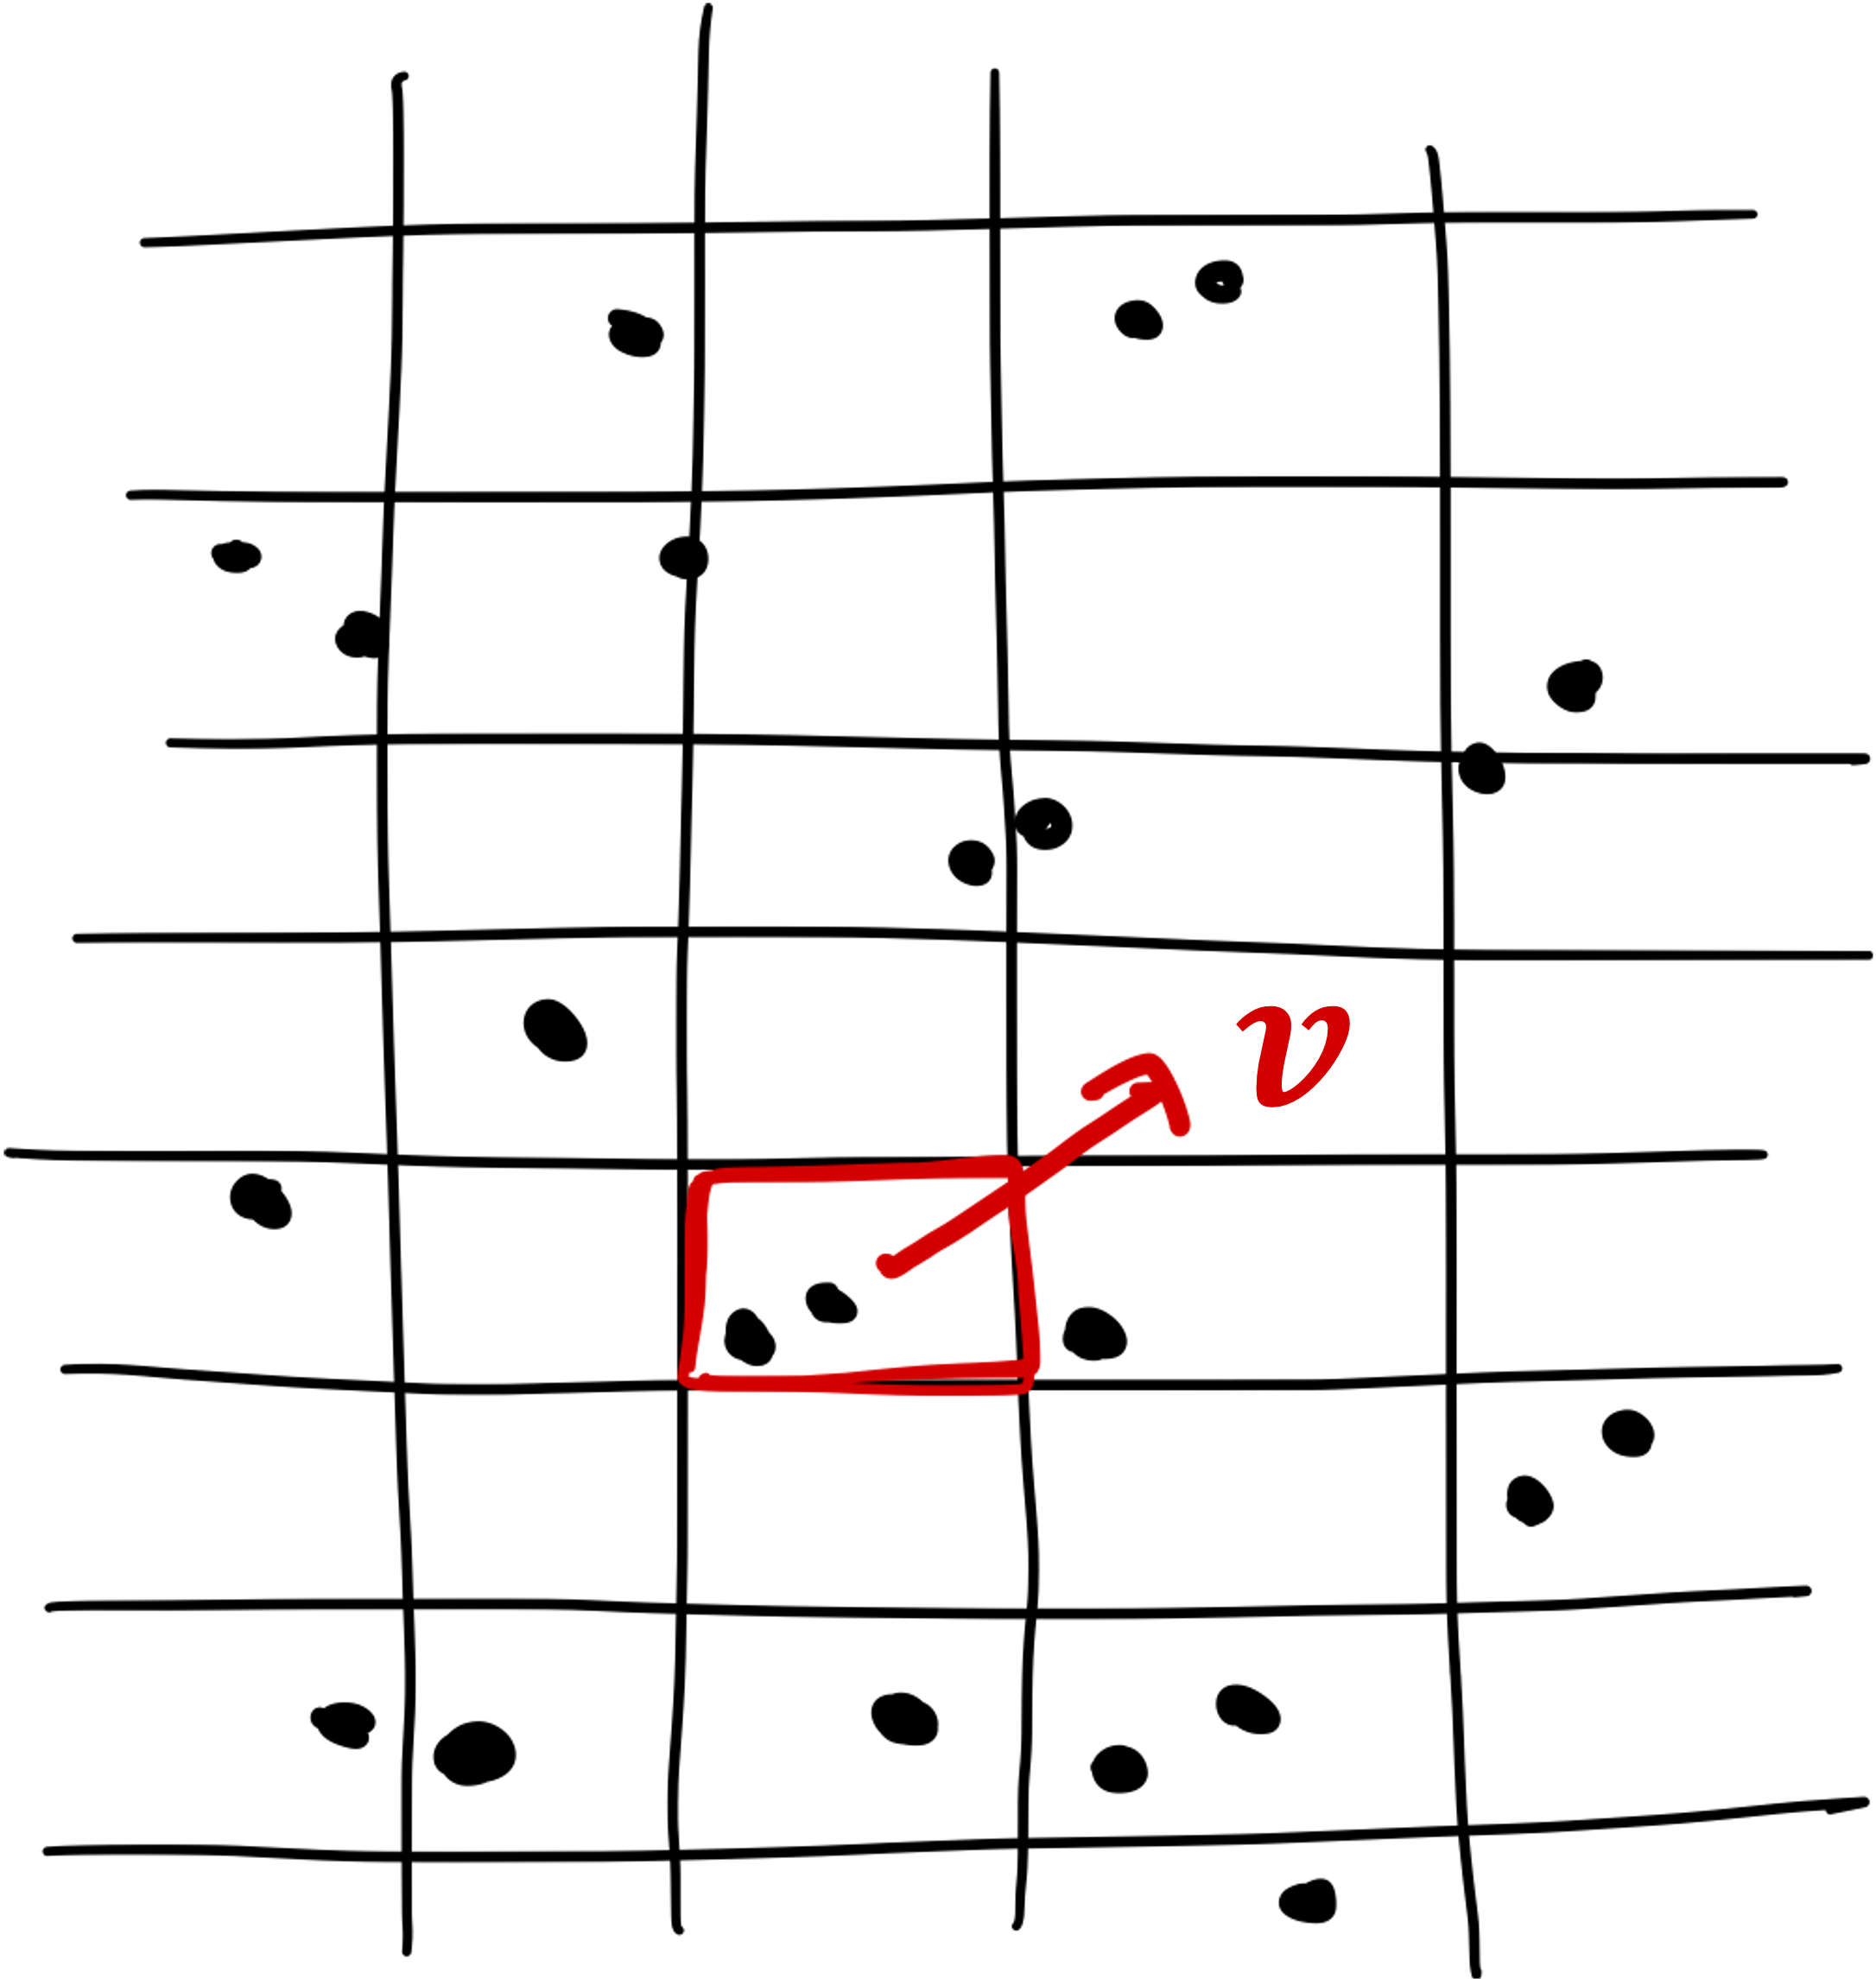
\includegraphics[width=\linewidth]{./pic/outflow_ex4.png}
		\subcaption{}
		\label{}
	\end{minipage}
	\begin{minipage}[b]{0.45\linewidth}
		\centering
		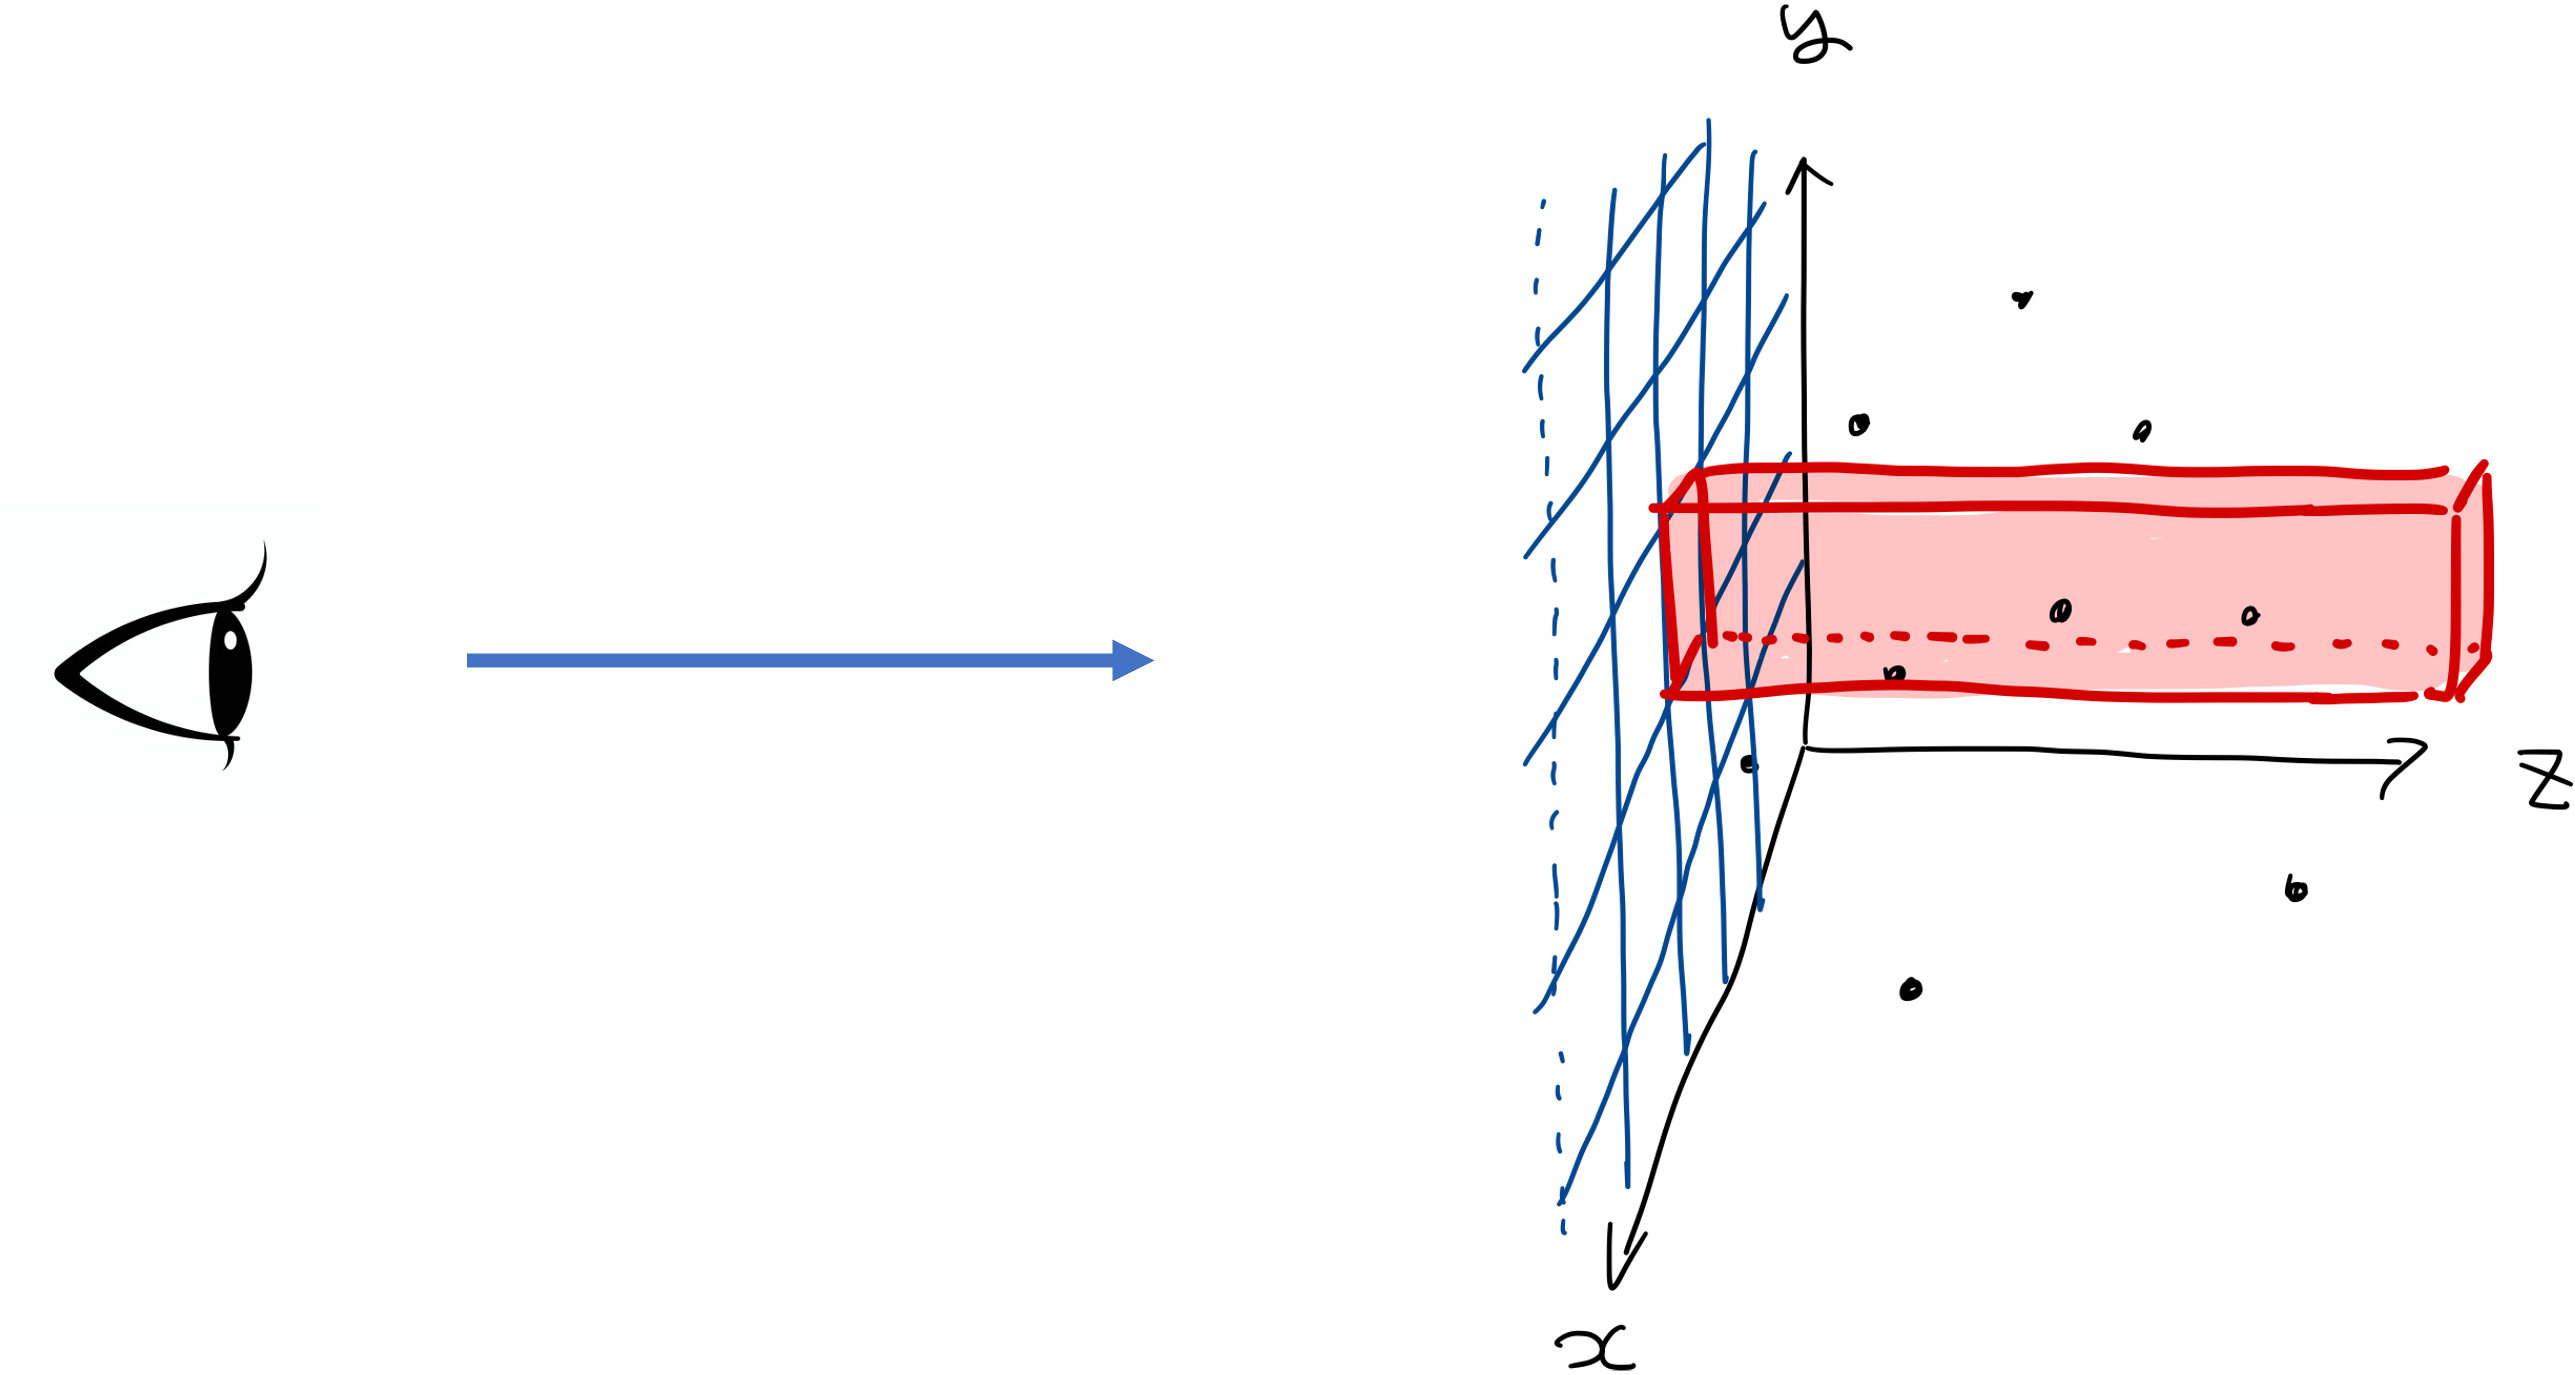
\includegraphics[width=\linewidth]{./pic/outflow_ex5.png}
		\subcaption{}
		\label{}
	\end{minipage}
	\captionsetup{width=0.9\linewidth}
	\caption{粒子やセルをメッシュ分けをして各メッシュの平均速度を導出しているイメージ図と$z$軸方向に対しても計算対象であることを示す図}
	\label{fig:calc_outflow}
\end{figure}

本論文においては,subhalo中心付近のみ射影(プロジェクション)を行い,なおアウトフローが確認できなかったものについて「アウトフローが確認できなかった」と表現している.